\begin{minipage}{0.75\linewidth}
\begin{figure}[h]
    \centering
    \begin{adjustbox}{max width=1.0\linewidth, keepaspectratio}
        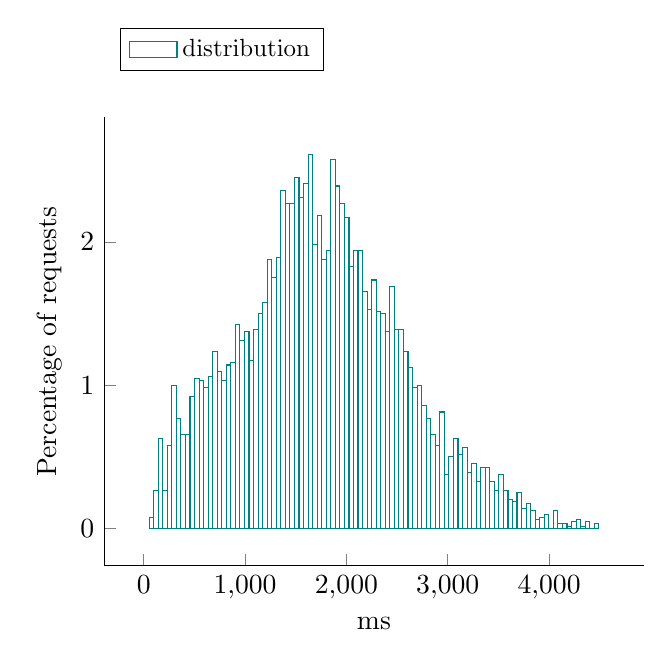
\begin{tikzpicture}
            \begin{axis}[ylabel = Percentage of requests, 
xlabel = ms, 
legend style = {nodes={scale=0.9, transform shape}, at={(0.03,1.2)}, anchor=north west, draw=black, fill=white, align=left, legend columns=3},
area style, mark size = 0pt,
 cycle list name = exotic,
  axis lines* = left]
		\addplot +[ybar interval] coordinates {
			 (53, 0.078125)
			 (97.82, 0.265625)
			 (142.64, 0.625)
			 (187.46, 0.265625)
			 (232.28, 0.578125)
			 (277.1, 1)
			 (321.92, 0.765625)
			 (366.74, 0.65625)
			 (411.56, 0.65625)
			 (456.38, 0.921875)
			 (501.2, 1.04688)
			 (546.02, 1.03125)
			 (590.84, 0.984375)
			 (635.66, 1.0625)
			 (680.48, 1.23438)
			 (725.3, 1.09375)
			 (770.12, 1.03125)
			 (814.94, 1.14062)
			 (859.76, 1.15625)
			 (904.58, 1.42188)
			 (949.4, 1.3125)
			 (994.22, 1.375)
			 (1039.04, 1.17188)
			 (1083.86, 1.39062)
			 (1128.68, 1.5)
			 (1173.5, 1.57812)
			 (1218.32, 1.875)
			 (1263.14, 1.75)
			 (1307.96, 1.89062)
			 (1352.78, 2.35938)
			 (1397.6, 2.26562)
			 (1442.42, 2.26562)
			 (1487.24, 2.45312)
			 (1532.06, 2.3125)
			 (1576.88, 2.40625)
			 (1621.7, 2.60938)
			 (1666.52, 1.98438)
			 (1711.34, 2.1875)
			 (1756.16, 1.875)
			 (1800.98, 1.9375)
			 (1845.8, 2.57812)
			 (1890.62, 2.39062)
			 (1935.44, 2.26562)
			 (1980.26, 2.17188)
			 (2025.08, 1.82812)
			 (2069.9, 1.9375)
			 (2114.72, 1.9375)
			 (2159.54, 1.65625)
			 (2204.36, 1.53125)
			 (2249.18, 1.73438)
			 (2294, 1.51562)
			 (2338.82, 1.5)
			 (2383.64, 1.375)
			 (2428.46, 1.6875)
			 (2473.28, 1.39062)
			 (2518.1, 1.39062)
			 (2562.92, 1.23438)
			 (2607.74, 1.125)
			 (2652.56, 0.984375)
			 (2697.38, 1)
			 (2742.2, 0.859375)
			 (2787.02, 0.765625)
			 (2831.84, 0.65625)
			 (2876.66, 0.578125)
			 (2921.48, 0.8125)
			 (2966.3, 0.375)
			 (3011.12, 0.5)
			 (3055.94, 0.625)
			 (3100.76, 0.515625)
			 (3145.58, 0.5625)
			 (3190.4, 0.390625)
			 (3235.22, 0.453125)
			 (3280.04, 0.328125)
			 (3324.86, 0.421875)
			 (3369.68, 0.421875)
			 (3414.5, 0.328125)
			 (3459.32, 0.265625)
			 (3504.14, 0.375)
			 (3548.96, 0.265625)
			 (3593.78, 0.203125)
			 (3638.6, 0.1875)
			 (3683.42, 0.25)
			 (3728.24, 0.140625)
			 (3773.06, 0.171875)
			 (3817.88, 0.125)
			 (3862.7, 0.0625)
			 (3907.52, 0.078125)
			 (3952.34, 0.09375)
			 (3997.16, 0)
			 (4041.98, 0.125)
			 (4086.8, 0.03125)
			 (4131.62, 0.03125)
			 (4176.44, 0.015625)
			 (4221.26, 0.046875)
			 (4266.08, 0.0625)
			 (4310.9, 0.015625)
			 (4355.72, 0.046875)
			 (4400.54, 0)
			 (4445.36, 0.03125)
			 (4490.18, 0.015625)
		};
\addlegendentry{distribution};
           \end{axis}
      \end{tikzpicture}
  \end{adjustbox}
  \caption{Response time distribution - req = ReadTimeline-2}
\end{figure}
\end{minipage}\hfill\begin{minipage}{0.18\linewidth}
\begin{table}[h]
\begin{tabular}{|cc|}
\hline
\textbf{} & \textbf{ms}\\ \hline
 \Xhline{0.005\arrayrulewidth}
min & 53\\
 \Xhline{0.005\arrayrulewidth}
max & 4535\\
 \Xhline{0.005\arrayrulewidth}
mean & 1757\\
 \Xhline{0.005\arrayrulewidth}
std & 806\\
\hline
\hline
 \Xhline{0.005\arrayrulewidth}
25th & 1209\\
 \Xhline{0.005\arrayrulewidth}
50th & 1724\\
 \Xhline{0.005\arrayrulewidth}
75th & 2275\\
 \Xhline{0.005\arrayrulewidth}
80th & 2429\\
 \Xhline{0.005\arrayrulewidth}
85th & 2582\\
 \Xhline{0.005\arrayrulewidth}
90th & 2810\\
 \Xhline{0.005\arrayrulewidth}
95th & 3198\\
 \Xhline{0.005\arrayrulewidth}
99th & 3766\\
\hline
\end{tabular}
\caption{Response time}
\end{table}
\end{minipage}\hfill